% Standard 3D Residual U-Net with SE Blocks Architecture Figure
% Compile with: pdflatex standard_unet_architecture.tex

\documentclass{article}
\usepackage[paperwidth=30cm, paperheight=12cm, margin=0.5cm]{geometry}
\usepackage{tikz}
\usepackage{xcolor}
\usepackage{amsmath}

\usetikzlibrary{shapes.geometric, arrows.meta, positioning, calc, backgrounds, fit, decorations.pathreplacing}

% Define colors (colorblind-friendly palette)
\definecolor{encoderblue}{RGB}{55, 126, 184}
\definecolor{decodergreen}{RGB}{77, 175, 74}
\definecolor{bottleneckorange}{RGB}{255, 127, 0}
\definecolor{skipgray}{RGB}{100, 100, 100}
\definecolor{inputgray}{RGB}{200, 200, 200}
\definecolor{seyellow}{RGB}{255, 193, 7}

\pagestyle{empty}

\begin{document}
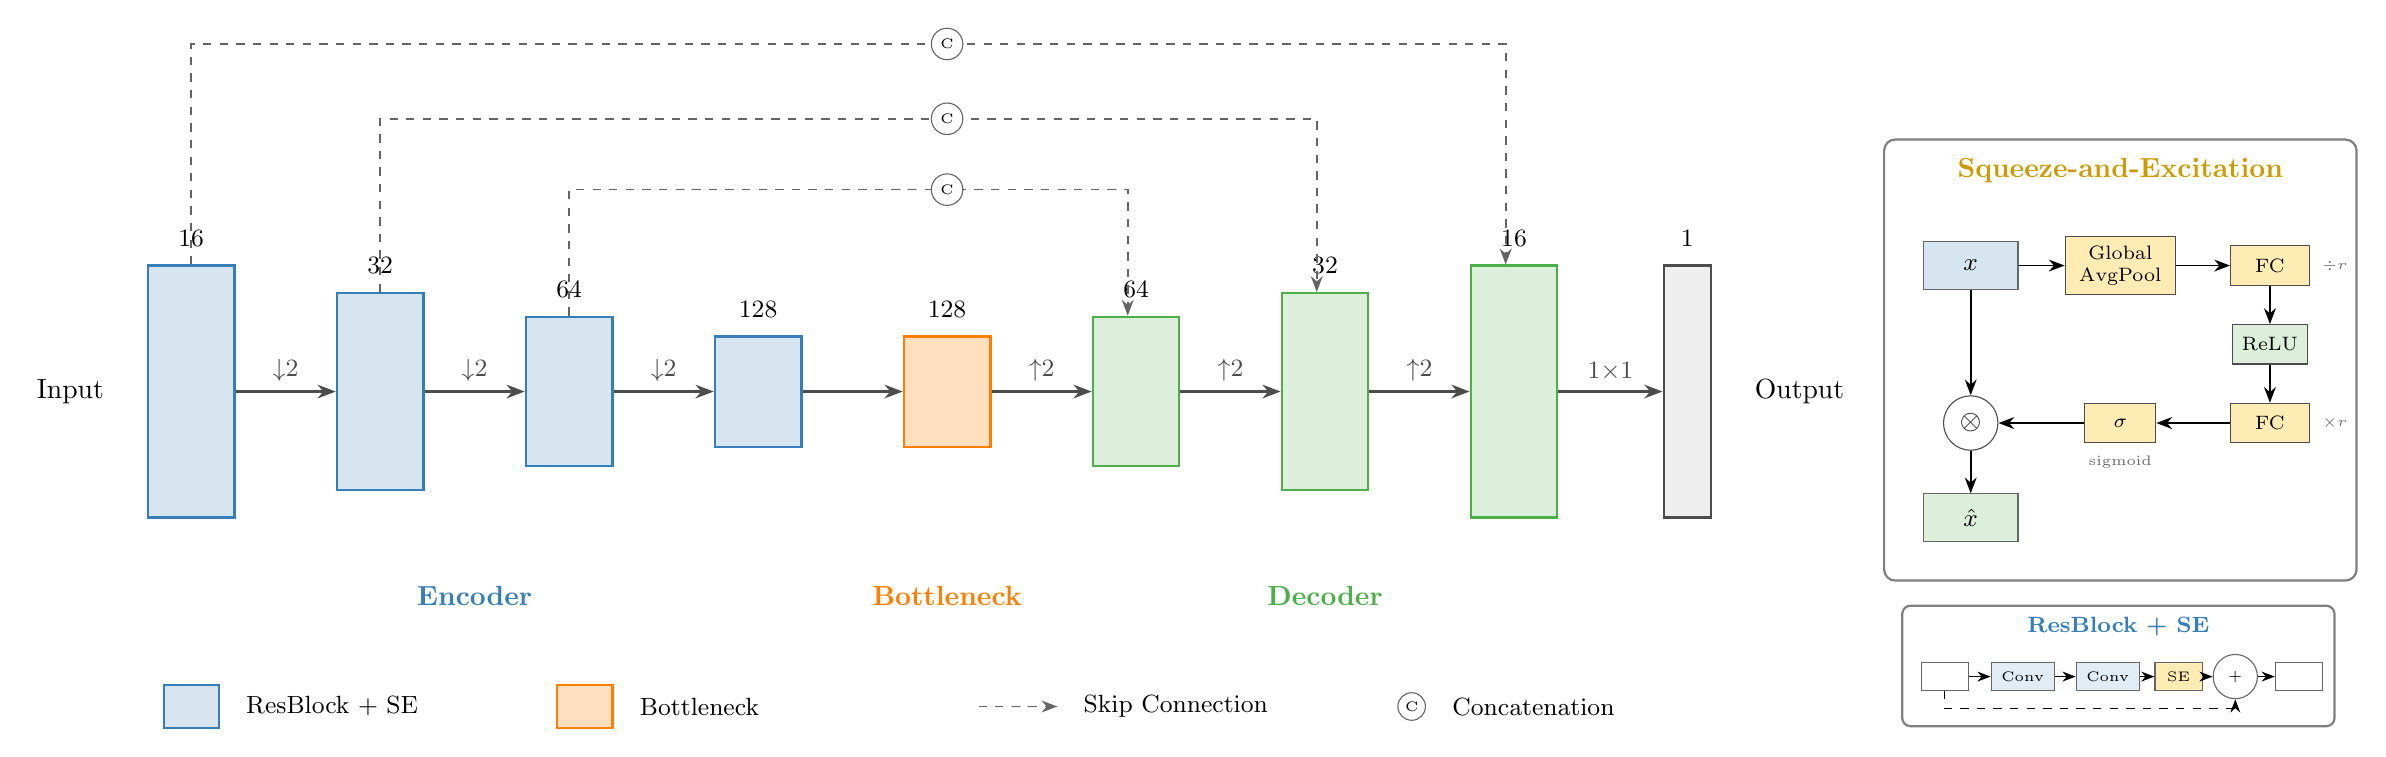
\begin{tikzpicture}[
    % Encoder block
    enc/.style={
        rectangle,
        draw=encoderblue,
        fill=encoderblue!20,
        line width=0.8pt,
        minimum width=1.1cm,
    },
    % Decoder block
    dec/.style={
        rectangle,
        draw=decodergreen,
        fill=decodergreen!20,
        line width=0.8pt,
        minimum width=1.1cm,
    },
    % Bottleneck block
    bottle/.style={
        rectangle,
        draw=bottleneckorange,
        fill=bottleneckorange!25,
        line width=0.8pt,
        minimum width=1.1cm,
    },
    % Output block
    outblock/.style={
        rectangle,
        draw=black!70,
        fill=inputgray!30,
        line width=0.8pt,
        minimum width=0.6cm,
    },
    % Arrow styles
    flow/.style={->, >=Stealth, thick, black!70},
    skip/.style={->, >=Stealth, semithick, skipgray, dashed},
    % Labels
    chanlabel/.style={font=\small, above=3pt},
    sublabel/.style={font=\tiny, text=black!60},
]

% =====================================================
% MAIN ARCHITECTURE
% =====================================================

% Encoder blocks (heights represent spatial dimensions)
\node[enc, minimum height=3.2cm] (e0) at (0, 0) {};
\node[enc, minimum height=2.5cm] (e1) at (2.4, 0) {};
\node[enc, minimum height=1.9cm] (e2) at (4.8, 0) {};
\node[enc, minimum height=1.4cm] (e3) at (7.2, 0) {};

% Channel labels
\node[chanlabel] at (e0.north) {16};
\node[chanlabel] at (e1.north) {32};
\node[chanlabel] at (e2.north) {64};
\node[chanlabel] at (e3.north) {128};

% Bottleneck (single block)
\node[bottle, minimum height=1.4cm] (btl) at (9.6, 0) {};
\node[chanlabel] at (btl.north) {128};

% Decoder blocks
\node[dec, minimum height=1.9cm] (d2) at (12.0, 0) {};
\node[dec, minimum height=2.5cm] (d1) at (14.4, 0) {};
\node[dec, minimum height=3.2cm] (d0) at (16.8, 0) {};

\node[chanlabel] at (d2.north) {64};
\node[chanlabel] at (d1.north) {32};
\node[chanlabel] at (d0.north) {16};

% Output
\node[outblock, minimum height=3.2cm] (out) at (19.0, 0) {};
\node[chanlabel] at (out.north) {1};

% =====================================================
% MAIN FLOW ARROWS
% =====================================================

% Encoder path
\draw[flow] (e0.east) -- (e1.west) node[midway, above, font=\small] {$\downarrow$2};
\draw[flow] (e1.east) -- (e2.west) node[midway, above, font=\small] {$\downarrow$2};
\draw[flow] (e2.east) -- (e3.west) node[midway, above, font=\small] {$\downarrow$2};
\draw[flow] (e3.east) -- (btl.west);

% Decoder path
\draw[flow] (btl.east) -- (d2.west) node[midway, above, font=\small] {$\uparrow$2};
\draw[flow] (d2.east) -- (d1.west) node[midway, above, font=\small] {$\uparrow$2};
\draw[flow] (d1.east) -- (d0.west) node[midway, above, font=\small] {$\uparrow$2};
\draw[flow] (d0.east) -- (out.west) node[midway, above, font=\small] {1$\times$1};

% =====================================================
% SKIP CONNECTIONS
% =====================================================

% Skip connection paths (encoder to decoder)
\draw[skip] (e2.north) -- ++(0, 1.6) -| ([xshift=-3pt]d2.north);
\draw[skip] (e1.north) -- ++(0, 2.2) -| ([xshift=-3pt]d1.north);
\draw[skip] (e0.north) -- ++(0, 2.8) -| ([xshift=-3pt]d0.north);

% Concat symbols
\node[circle, draw=skipgray, fill=white, minimum size=0.4cm, font=\tiny, inner sep=0pt] at ($(e2.north) + (4.8, 1.6)$) {C};
\node[circle, draw=skipgray, fill=white, minimum size=0.4cm, font=\tiny, inner sep=0pt] at ($(e1.north) + (7.2, 2.2)$) {C};
\node[circle, draw=skipgray, fill=white, minimum size=0.4cm, font=\tiny, inner sep=0pt] at ($(e0.north) + (9.6, 2.8)$) {C};

% =====================================================
% INPUT/OUTPUT LABELS
% =====================================================

\node[left=12pt of e0, font=\normalsize] {Input};
\node[right=12pt of out, font=\normalsize] {Output};

% Section labels
\node[font=\normalsize\bfseries, encoderblue] at (3.6, -2.6) {Encoder};
\node[font=\normalsize\bfseries, bottleneckorange] at (9.6, -2.6) {Bottleneck};
\node[font=\normalsize\bfseries, decodergreen] at (14.4, -2.6) {Decoder};

% =====================================================
% SE BLOCK INSET
% =====================================================

\begin{scope}[shift={(22.0, 0.8)}, scale=1.0]
    % Inset box
    \draw[black!50, thick, rounded corners=4pt] (-0.5, -3.2) rectangle (5.5, 2.4);
    \node[font=\normalsize\bfseries, seyellow!80!black] at (2.5, 2.0) {Squeeze-and-Excitation};

    % Input
    \node[rectangle, draw=black!60, fill=encoderblue!20, minimum width=1.2cm, minimum height=0.6cm, font=\small] (se_in) at (0.6, 0.8) {$x$};

    % Global Average Pool
    \node[rectangle, draw=black!70, fill=seyellow!30, minimum width=1.4cm, minimum height=0.6cm, font=\scriptsize, align=center] (gap) at (2.5, 0.8) {Global\\AvgPool};

    % FC1
    \node[rectangle, draw=black!70, fill=seyellow!30, minimum width=1.0cm, minimum height=0.5cm, font=\scriptsize] (fc1) at (4.4, 0.8) {FC};

    % ReLU
    \node[rectangle, draw=black!70, fill=decodergreen!20, minimum width=0.8cm, minimum height=0.5cm, font=\scriptsize] (relu) at (4.4, -0.2) {ReLU};

    % FC2
    \node[rectangle, draw=black!70, fill=seyellow!30, minimum width=1.0cm, minimum height=0.5cm, font=\scriptsize] (fc2) at (4.4, -1.2) {FC};

    % Sigmoid
    \node[rectangle, draw=black!70, fill=seyellow!30, minimum width=0.9cm, minimum height=0.5cm, font=\scriptsize] (sig) at (2.5, -1.2) {$\sigma$};

    % Multiply
    \node[circle, draw=black!70, fill=white, minimum size=0.5cm, font=\normalsize] (mul) at (0.6, -1.2) {$\otimes$};

    % Output
    \node[rectangle, draw=black!60, fill=decodergreen!20, minimum width=1.2cm, minimum height=0.6cm, font=\small] (se_out) at (0.6, -2.4) {$\hat{x}$};

    % Arrows
    \draw[->, >=Stealth, semithick] (se_in) -- (gap);
    \draw[->, >=Stealth, semithick] (gap) -- (fc1);
    \draw[->, >=Stealth, semithick] (fc1) -- (relu);
    \draw[->, >=Stealth, semithick] (relu) -- (fc2);
    \draw[->, >=Stealth, semithick] (fc2) -- (sig);
    \draw[->, >=Stealth, semithick] (sig) -- (mul);
    \draw[->, >=Stealth, semithick] (mul) -- (se_out);

    % Skip connection from input to multiply
    \draw[->, >=Stealth, semithick] (se_in.south) -- ++(0, -0.5) -| (mul.north);

    % Labels
    \node[font=\tiny, text=black!60, right=1pt of fc1] {$\div r$};
    \node[font=\tiny, text=black!60, right=1pt of fc2] {$\times r$};
    \node[font=\tiny, text=black!60, below=1pt of sig] {sigmoid};
\end{scope}

% =====================================================
% RESIDUAL BLOCK DETAIL (small)
% =====================================================

\begin{scope}[shift={(22.0, -3.8)}, scale=0.9]
    \draw[black!50, thick, rounded corners=3pt] (-0.3, -0.5) rectangle (5.8, 1.2);
    \node[font=\footnotesize\bfseries, encoderblue] at (2.75, 0.9) {ResBlock + SE};

    \node[rectangle, draw=black!60, fill=white, minimum width=0.6cm, minimum height=0.35cm, font=\tiny] (rb_in) at (0.3, 0.2) {};
    \node[rectangle, draw=black!60, fill=encoderblue!15, minimum width=0.8cm, minimum height=0.35cm, font=\tiny] (conv1) at (1.4, 0.2) {Conv};
    \node[rectangle, draw=black!60, fill=encoderblue!15, minimum width=0.8cm, minimum height=0.35cm, font=\tiny] (conv2) at (2.6, 0.2) {Conv};
    \node[rectangle, draw=black!60, fill=seyellow!30, minimum width=0.6cm, minimum height=0.35cm, font=\tiny] (se) at (3.6, 0.2) {SE};
    \node[circle, draw=black!60, fill=white, minimum size=0.3cm, font=\tiny] (add) at (4.4, 0.2) {$+$};
    \node[rectangle, draw=black!60, fill=white, minimum width=0.6cm, minimum height=0.35cm, font=\tiny] (rb_out) at (5.3, 0.2) {};

    \draw[->, >=Stealth, thin] (rb_in) -- (conv1);
    \draw[->, >=Stealth, thin] (conv1) -- (conv2);
    \draw[->, >=Stealth, thin] (conv2) -- (se);
    \draw[->, >=Stealth, thin] (se) -- (add);
    \draw[->, >=Stealth, thin] (add) -- (rb_out);
    \draw[->, >=Stealth, thin, dashed] (rb_in.south) -- ++(0, -0.25) -| (add.south);
\end{scope}

% =====================================================
% LEGEND
% =====================================================

\begin{scope}[shift={(0, -4.0)}]
    % ResBlock + SE
    \node[enc, minimum height=0.55cm, minimum width=0.7cm] (l1) at (0, 0) {};
    \node[font=\small, right=6pt of l1] {ResBlock + SE};

    % Bottleneck
    \node[bottle, minimum height=0.55cm, minimum width=0.7cm] (l2) at (5.0, 0) {};
    \node[font=\small, right=6pt of l2] {Bottleneck};

    % Skip connection
    \draw[skip] (10.0, 0) -- ++(1.0, 0);
    \node[font=\small, right=6pt] at (11.0, 0) {Skip Connection};

    % Concat
    \node[circle, draw=skipgray, fill=white, minimum size=0.35cm, font=\tiny, inner sep=0pt] (l4) at (15.5, 0) {C};
    \node[font=\small, right=6pt of l4] {Concatenation};
\end{scope}

\end{tikzpicture}
\end{document}
